\documentclass{article}

\usepackage{graphicx}
\usepackage{multicol}
\usepackage[margin=0.5in]{geometry}
\usepackage{ragged2e}
\usepackage{boondox-cal}
\usepackage[export]{adjustbox}
\usepackage{wrapfig}
\renewcommand{\vec}[1]{\mathbf{#1}}

\begin{document}


\title{Engineering Design I - Crosswalk Traffic Controller}
\author{Joseph Spear}

\maketitle


\section{Problem}
At Austin Peay State University, vehicle and pedestrian traffic can sometimes interfere with each other in inefficient or even dangerous ways. Therefore, it is especially important to take detailed considerations of intersections like crosswalks. We have been tasked with developing a traffic control system for the crosswalk on Eighth street between Sundquist and Maynard. The system should provide the following:

\begin{itemize}
\item{Clear and accurate signals for pedestrians and vehicles to prioritize safety and meet local, state and federal traffic control requirements.}
\item{Will prevent backups at the intersection of Eighth and College.}
\item{Pedestrians shall not wait for more than one minute.}
\item{Take into consideration the traffic flow from the Trahern parking lot.}
\item{Active detection of the presence of pedestrians and vehicles.}
\end{itemize}



\section{Research and Data Collection}
\subsection{Crosswalk Regulations}
Laws regarding crosswalks for the State of Tennessee are:

\begin{itemize}
\item T.C.A.  55-8-134: When traffic signal is not in place, vehicles must yield to pedestrian in crosswalk on vehicle’s half of road or close to it. Pedestrians must not step off curb and into path of vehicle when vehicle does not have time to stop.

\item T.C.A.  55-8-197: Any person that injures or kills a pedestrian while violating T.C.A. 55-8-134 is guilty of a misdemeanor.

\item T.C.A.  55-8-135: Pedestrians must yield to vehicles when crossing outside crosswalk. Pedestrians must use crosswalk at intersections with traffic control devices.

\end{itemize}


\subsection{Traffic Observation}
When determining the traffic flow rate, it is important to determine the highest velocity situation and make sure the system can accommodate this. The hypothetical highest velocity would occur at class changes for pedestrians, and 7-9AM/4-6PM for vehicles. This is the assumption for the traffic flow velocities. Below is a sample of data gathered for analysis of the volume flow.

\begin{table}[h!]
  \begin{center}
    \caption{Traffic Flow Rate}
    \label{tab:table1}
    \begin{tabular}{l|c|c}
      \textbf{Time} & \textbf{Pedestrian Rate $\left(Minute^{-1}\right)$} & \textbf{Traffic Rate $\left(Minute^{-1}\right)$}\\
      \hline
      9:57AM & 3 & 2\\
      9:59AM & 3 & 4\\
      10:01AM & 3 & 4\\
      10:03AM & 3 & 3\\
      10:05AM & 6 & 5\\
      10:07AM & 5 & 3\\
      10:09AM & 3 & 6
    \end{tabular}
  \end{center}
\end{table}

\vspace{2in}

The above data was collected on Wednesday, November 18th 2020. The gathered data is assumed to be significantly reduced in comparison to a typical day due to the low in-class attendance caused by COVID-19.

The total distance from College Street to the crosswalk is roughly 330ft. Assuming a car-length and gap distance of 20 ft, about 16 vehicles may be able to be waiting before this becomes a problem. Given the information in Table 1, it is safe to say that this will not be surpassed in the time it takes for the cycle to get back to allowing vehicles to pass through. A similar distance is found for the distance between Jackson Alley and the crosswalk.


\section{Traffic Control Process}
The design of traffic system is defined in terms of States, Transitions, Conditions, and Sequences.

\begin{itemize}

\item \underline{State} - State is used to describe the configuration of the various traffic lights.
\item \underline{Transition} - Transition is used to describe the process to change from one state to another.
\item \underline{Condition} - The situation which determines the State. Changing Conditions determine which Transition to use.
\item \underline{Sequence} - An ordering of various transitions to produce a traffic cycle based on an initial condition.

\end{itemize}

When analyzing the situation, states and transitions are used to determine the best course of action for the control system, based on the provided conditions. There are 6 major states as shown in figure 1.

\begin{center}
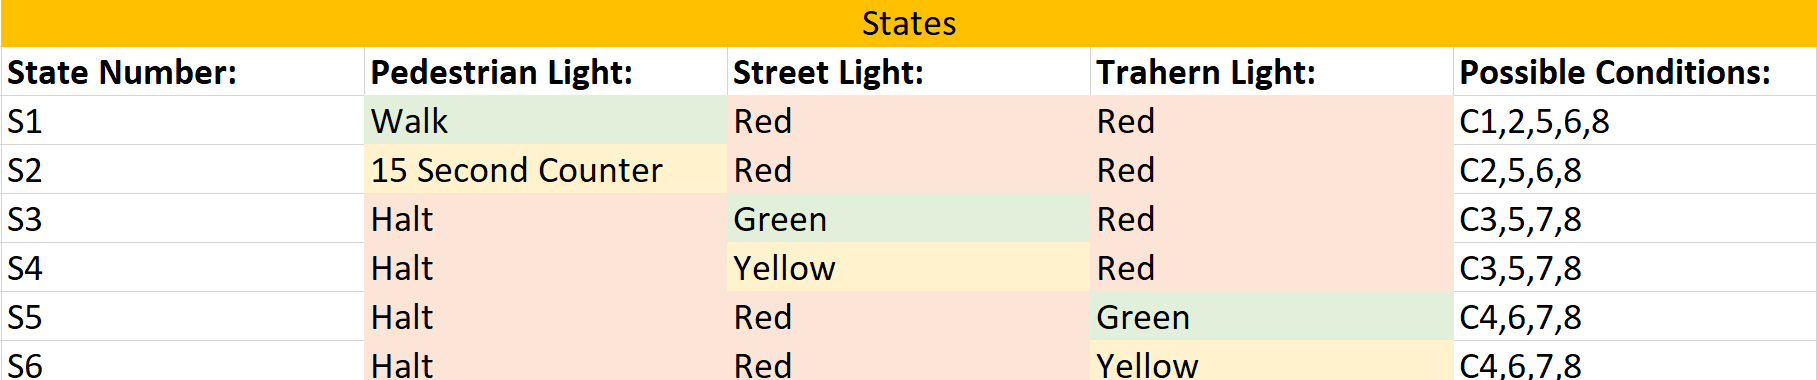
\includegraphics[width=0.85\linewidth, center]{States.png}
\scriptsize{
Figure 1: Table of States and their descriptions.
}
\end{center}

It should also be known that there is an implied State after every State that includes a yellow light. This state is where all lights are red for 3 seconds.

The Conditions are essentially variables used to determine which State the system needs to be in. There are 3 conditions, each of which having 2 responses as depicted below in figure 2.

\begin{center}
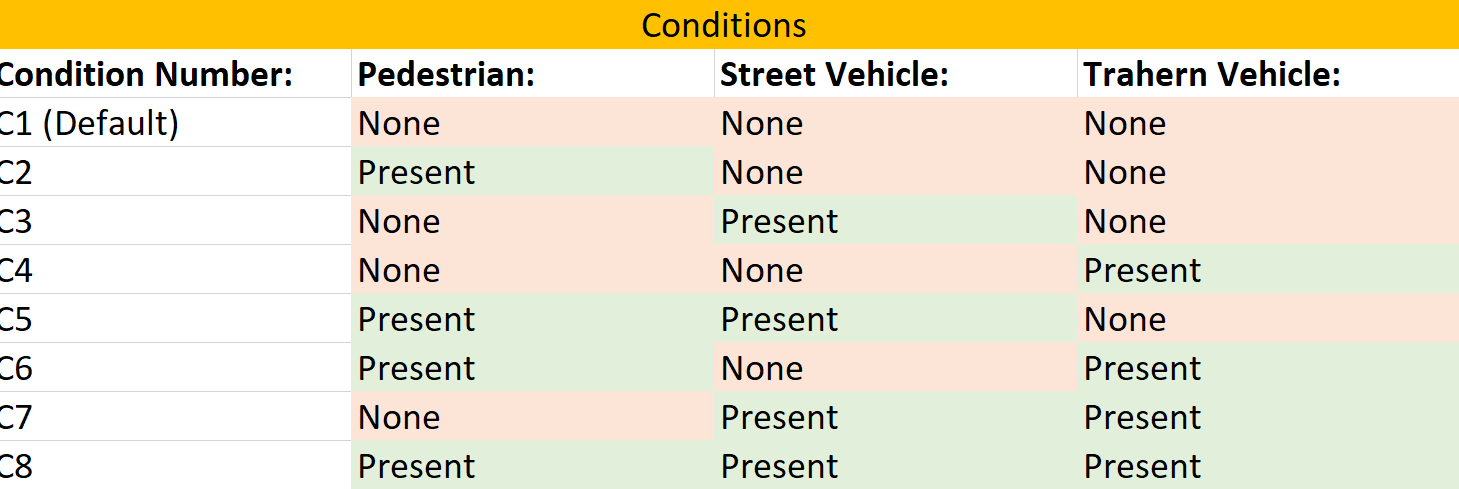
\includegraphics[width=0.85\linewidth, center]{Conditions.png}
\scriptsize{
Figure 2: Table of Possible Conditions.
}
\end{center}

Each Condition represents a possible situation that the system must take into account to determine which State it would most efficiently work in.

The Transitions are the processes in which the system moves between States. For example, a 25 second time limit is set on the pedestrian light when it first turns green, and when elapsed, a signal will be emitted for the pedestrian light to switch from the green State (Walk) to the yellow State (15 Second Countdown). The entire listing of Transitions is shown in figure 3.

\begin{center}
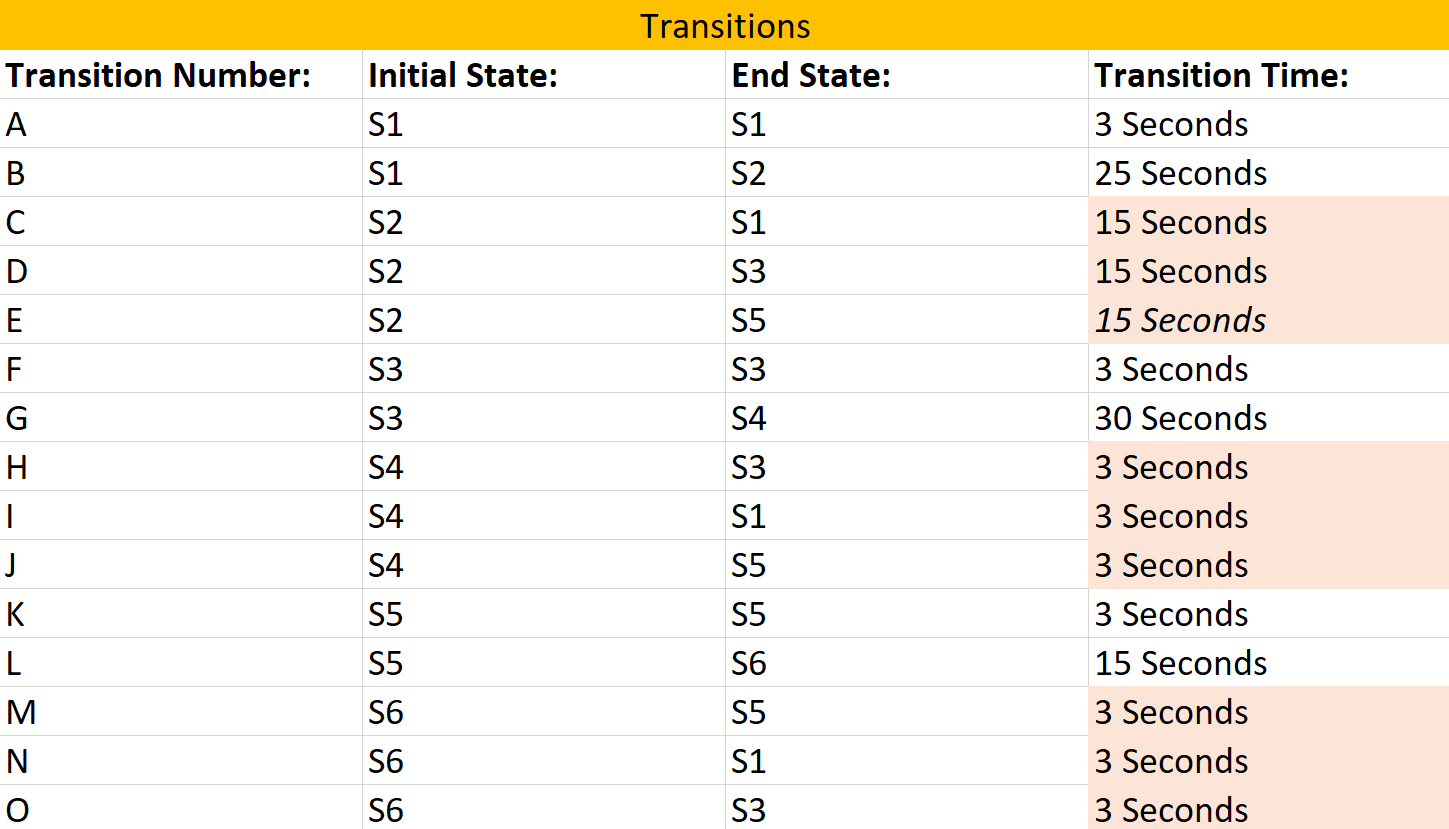
\includegraphics[width=0.85\linewidth, center]{Transitions.png}
\scriptsize{
Figure 3: Transitions Table.
}
\end{center}

\subsection{Process Sequence Diagram}

Taking into account figures 1,2, and 3, we can determine all possible situations and all possible transitions to maintain a continuous and efficient traffic cycle. Figure 4 shows the process flow diagram, with the initial State being State 1 (Pedestrian Light is green, other lights are red).


\begin{center}
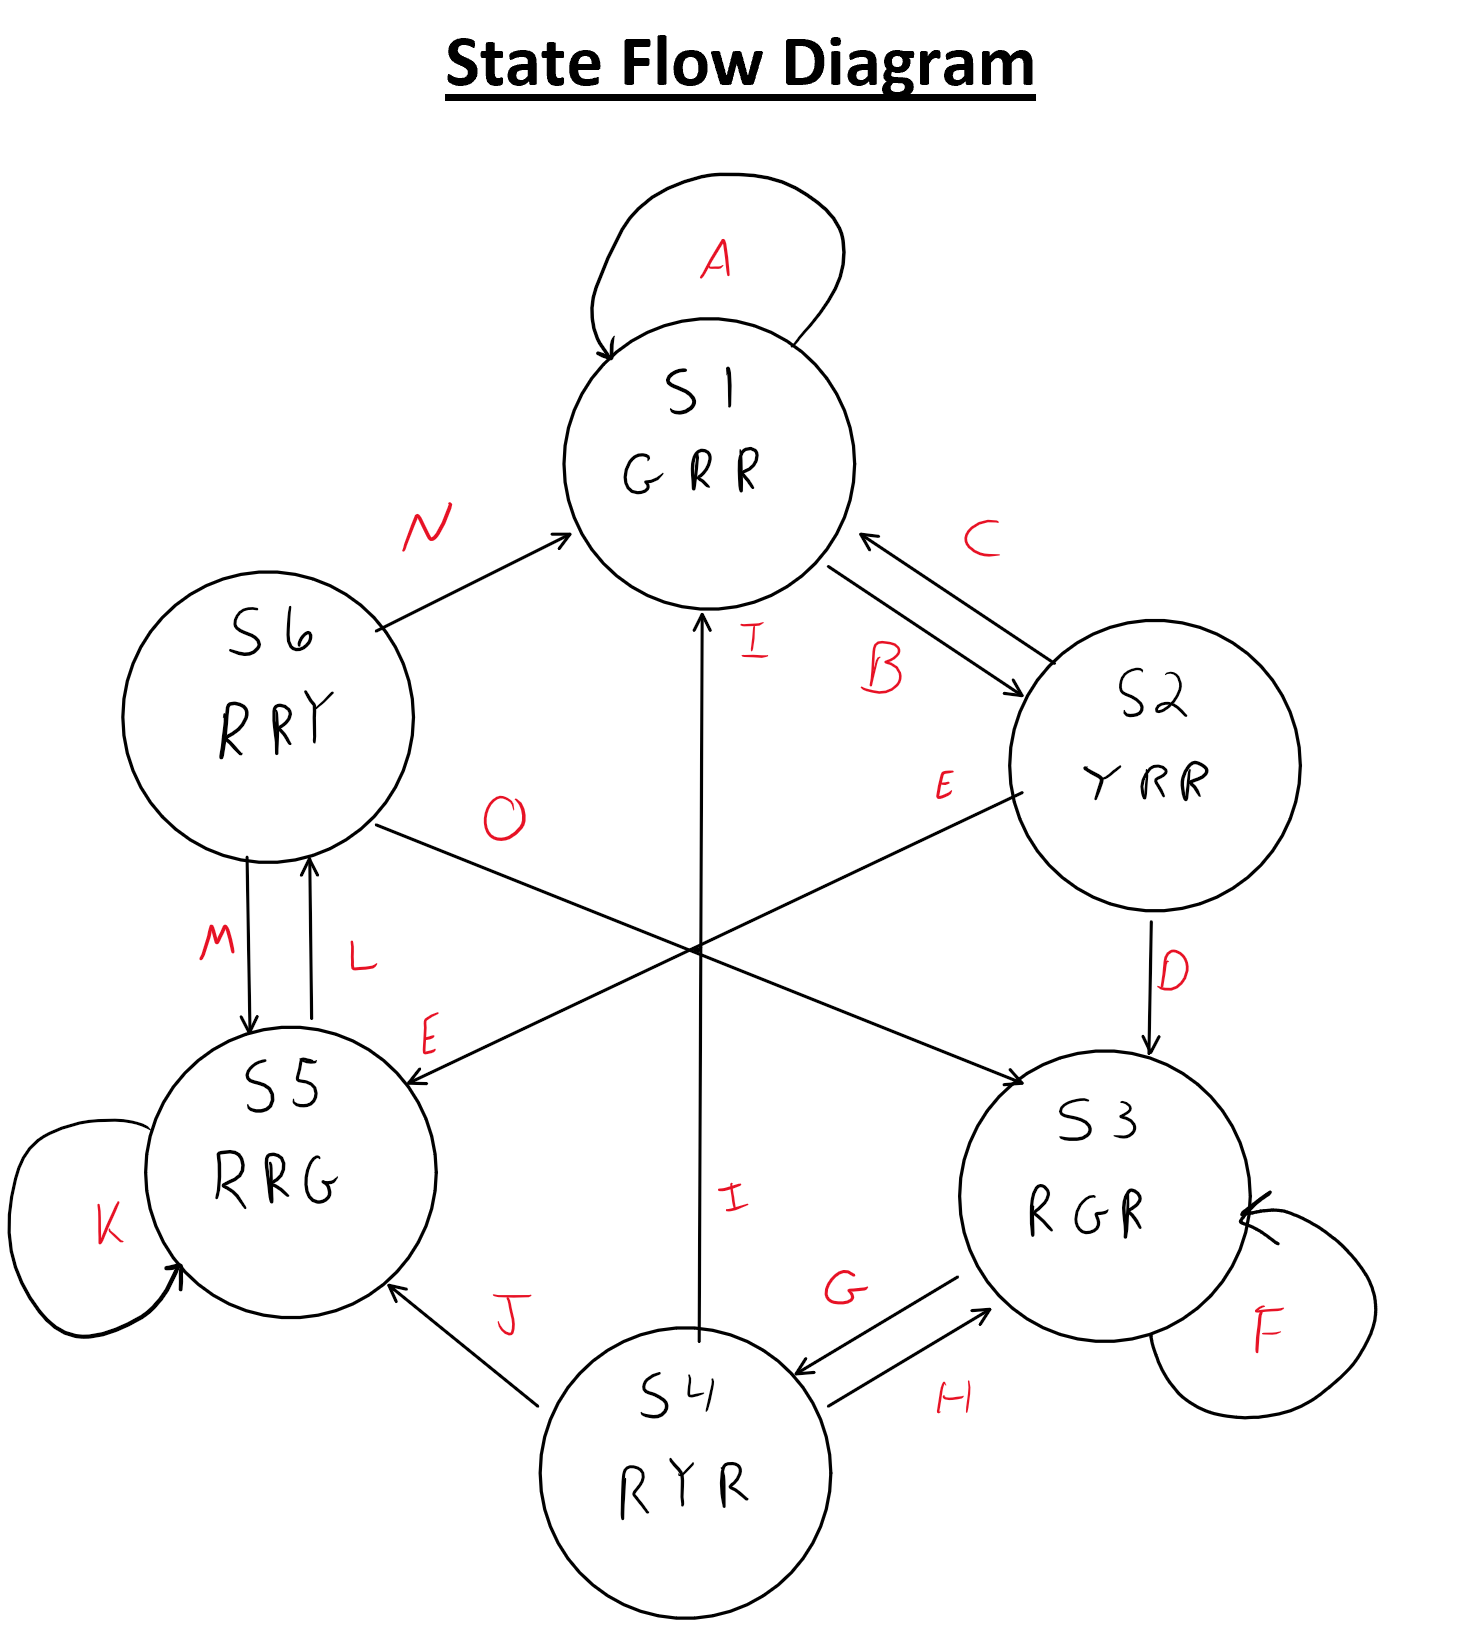
\includegraphics[width=0.5\textwidth, center]{State_Flow_Diagram.png}
\scriptsize{
Figure 4a: Diagram showing the Sequence Flow.
}
\end{center}

\begin{center}
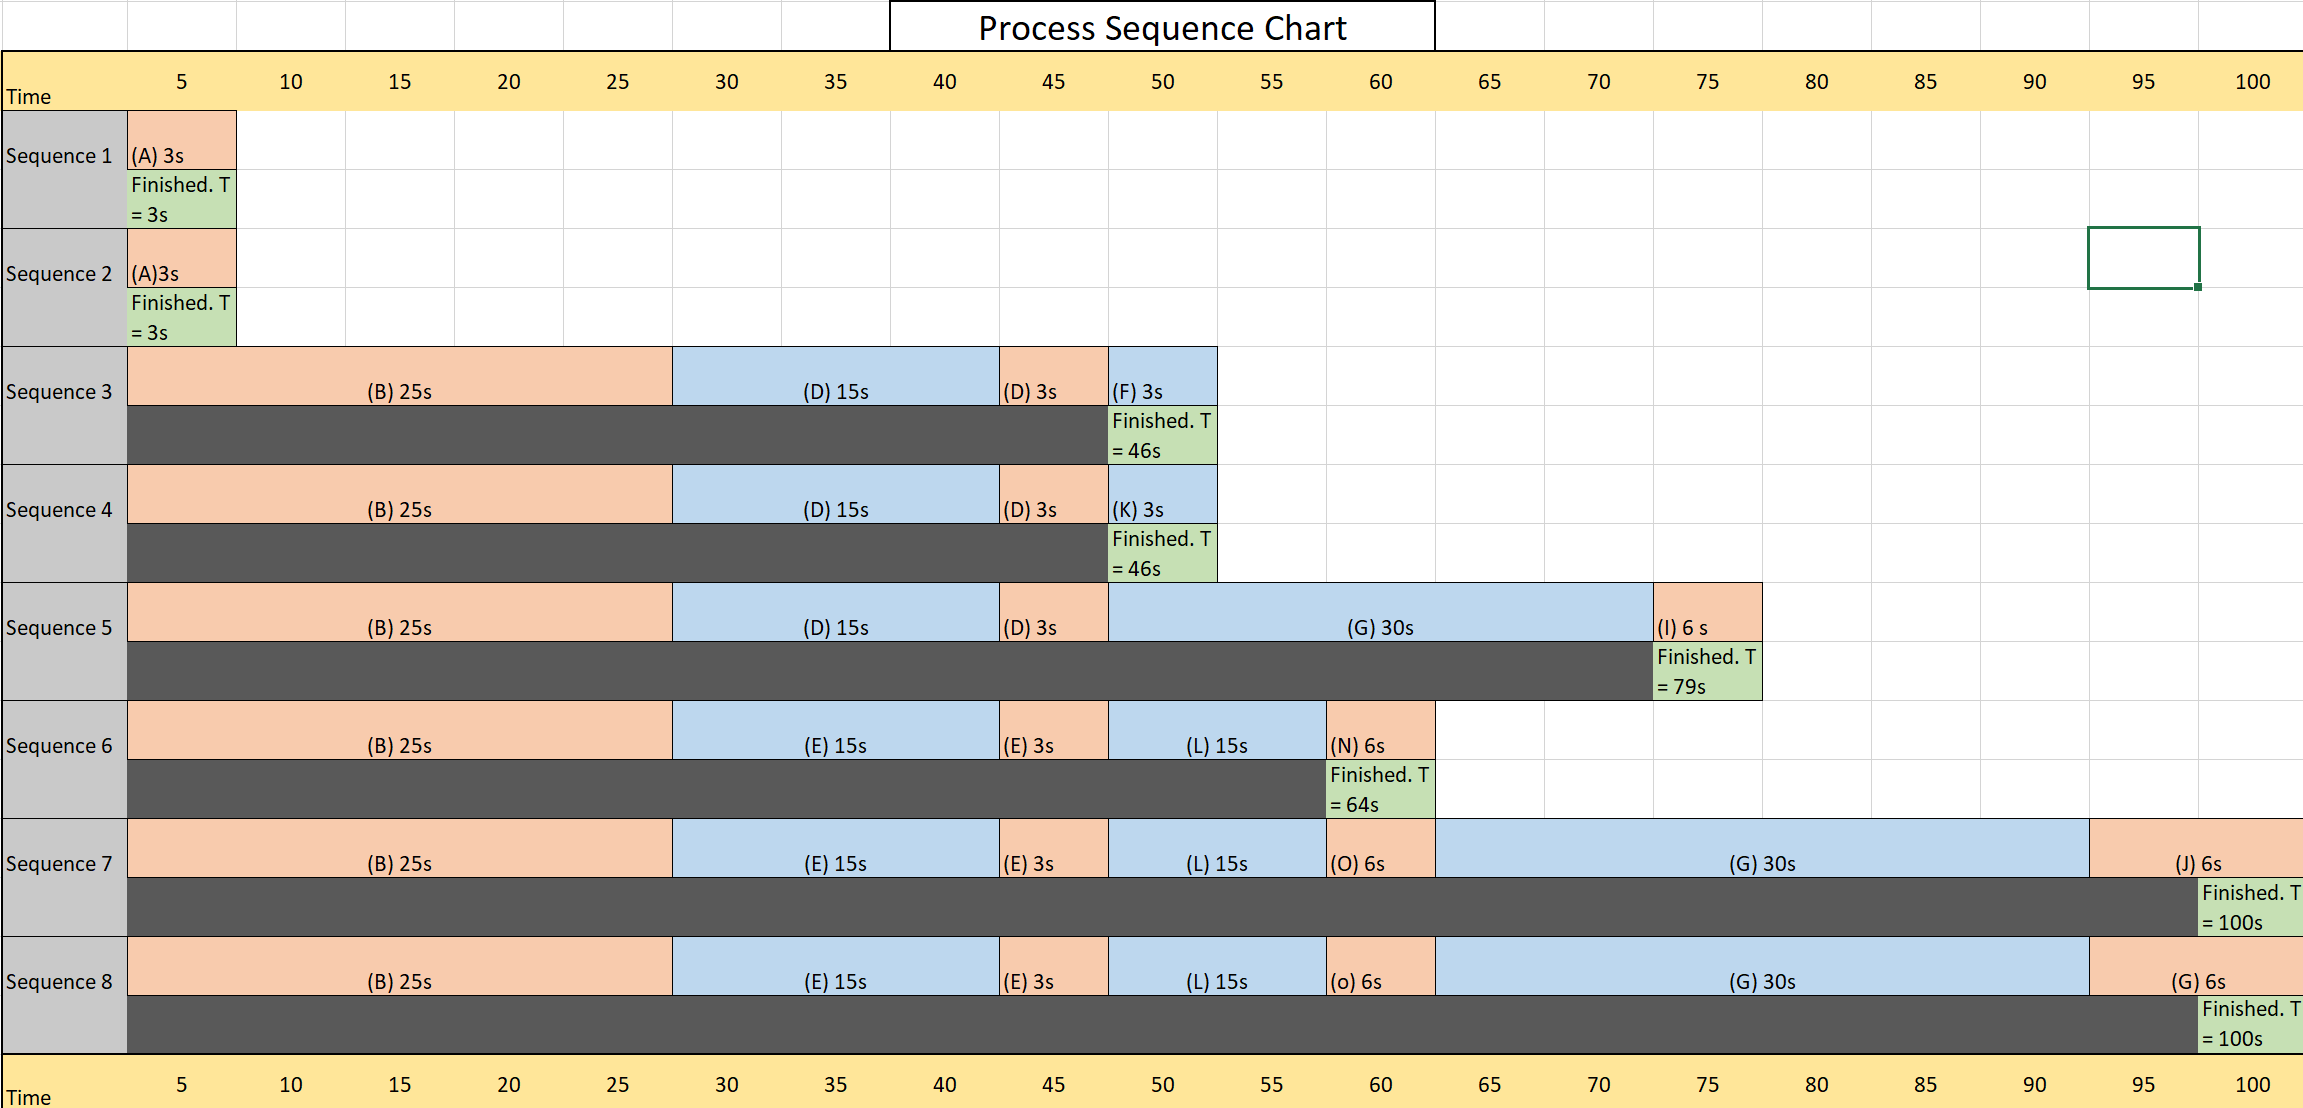
\includegraphics[width=0.85\textwidth, center]{ProcessSequenceChart.png}
\scriptsize{
Figure 4b: Process Sequence Chart.
}
\end{center}


In order to ensure that each Condition has a an efficient cycle, a Sequence of Transitions will be used once a Condition is met. These Sequences run repeatedly until the Condition changes. Figure 5 shows a listing of all the possible Sequences for the given Conditions.

\begin{center}
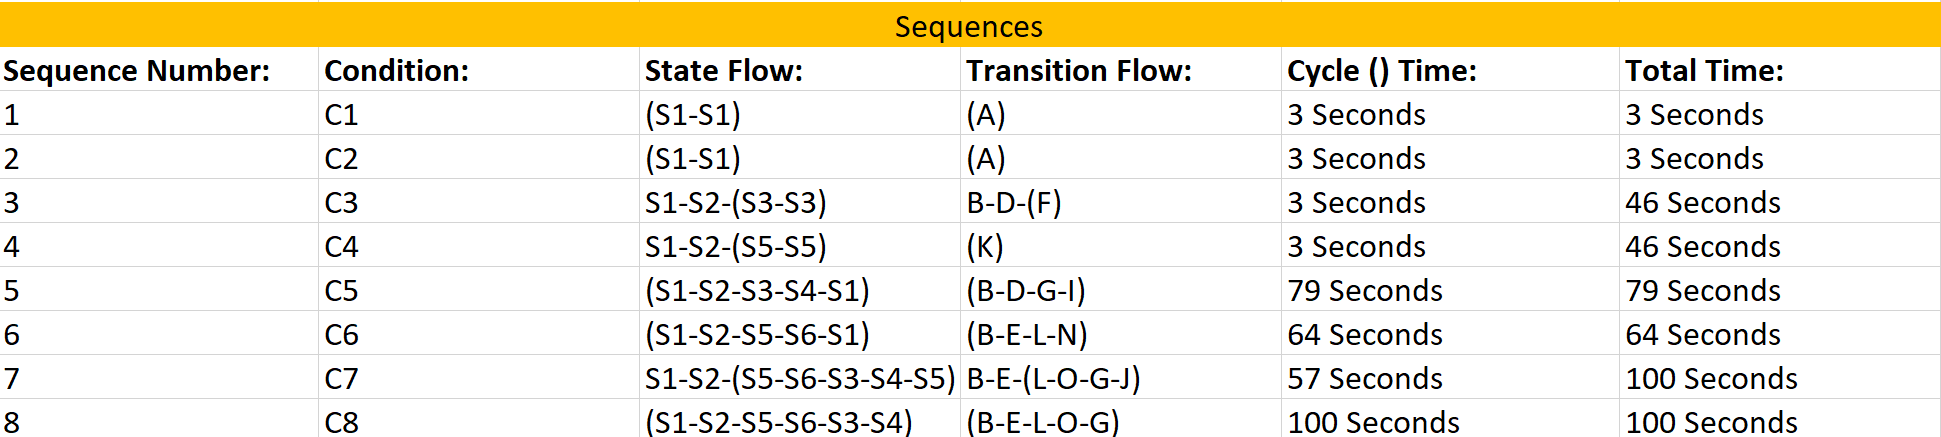
\includegraphics[width=0.9\textwidth, center]{Sequences.png}
\scriptsize{
Figure 5: Table of Sequences.
}
\end{center}

\section{System}
The basic layout of the traffic system is given below. The key component in the design is the Arduino Duo, which is the micro-controller used to send output signals to the system based on the readings of the input signals provided by the inferred sensors. The States, Transitions, Conditions, and Sequences would all be coded in the Arduino as instructions on how to efficiently operate the traffic system.

In order to provide necessary power, the power from the grid has to be converted to DC power using a converter. This DC power is stepped down in voltage using a transformer and then used by the Arduino for signal processing. The Arduino intakes signals from the inferred sensors when either a pedestrian or vehicle is detected respectively, and this changes the Conditions for the system. Depending on the Conditions, a specific signal will be sent at the moment a Transition occurs, changing the State of the system. 

\begin{center}
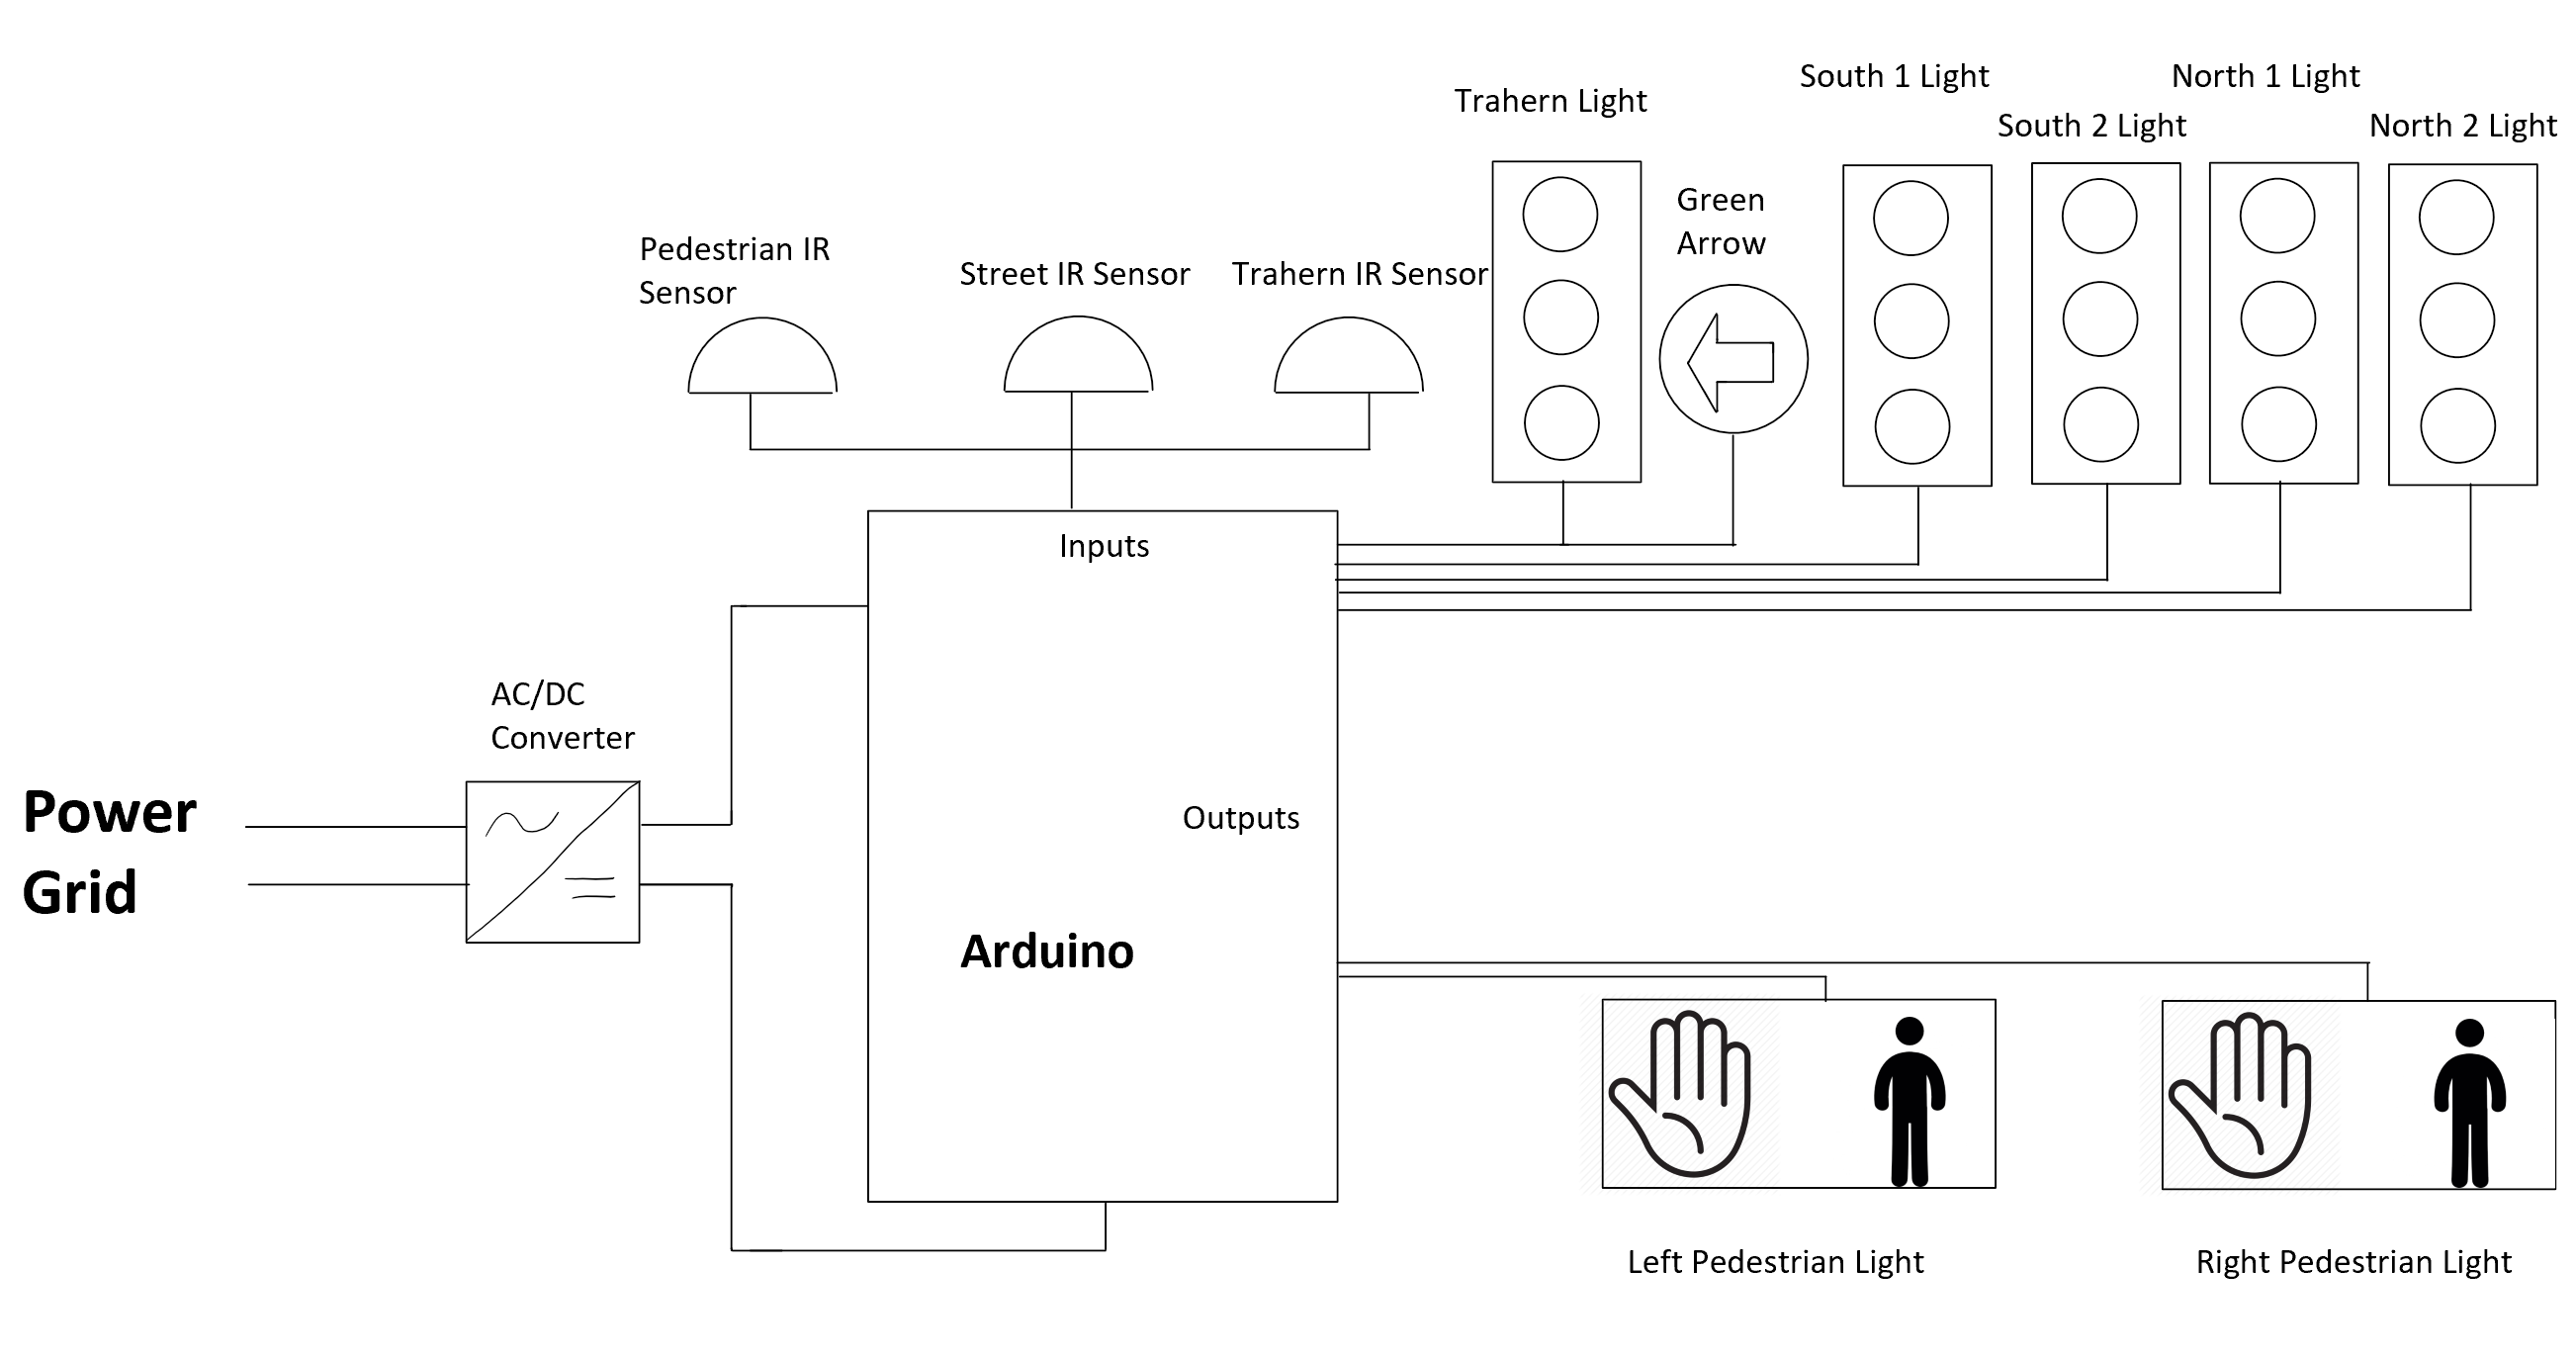
\includegraphics[width=0.9\textwidth, center]{CircuitDesign.png}
\scriptsize{
Figure 6: Basic Circuit Diagram.
}
\end{center}



\section{Installation}
\begin{wrapfigure}{5}{0.25\textwidth}
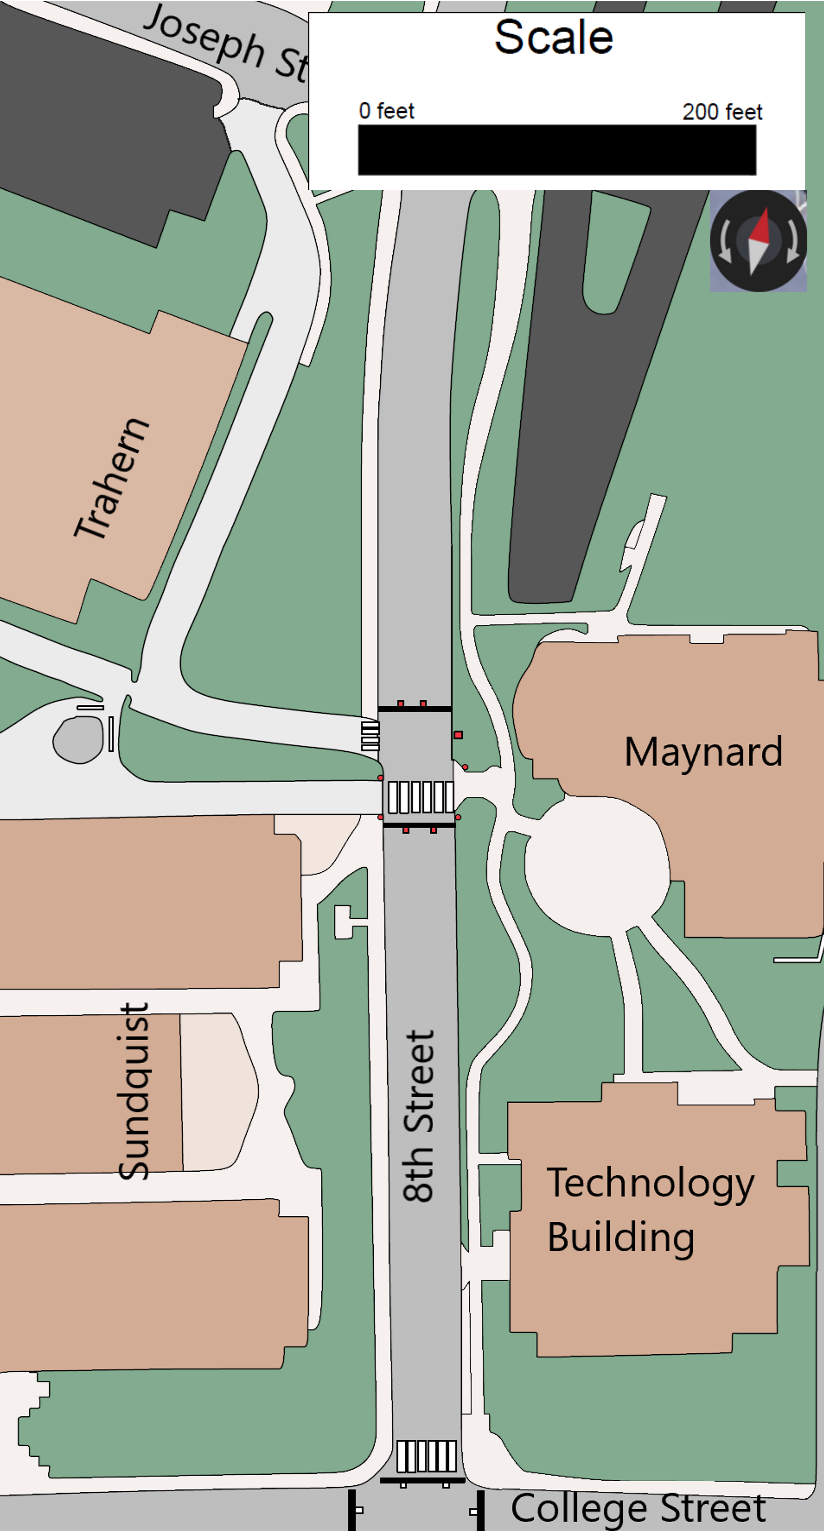
\includegraphics[width=\linewidth]{MapWithScale.png} 
\begin{center}
\scriptsize{
Figure 7: Site Map of 8th and College Street (421' x 799').
}
\end{center}
\end{wrapfigure}

When it is desired to install civil infrastructure, it is necessary to have an understanding of the surrounding area. Having this knowledge provides a broad scope for any issues that could arise during the installation or post-installation. \vspace{0.075in}

Figure 7 provides a 421' x 799' surrounding area of the crosswalk in question. It provides the location of the crosswalk, College Street, Joseph Street, surrounding buildings and parking lots, and the theorized traffic lights, colored in bright red around the crosswalk. This image was produced using Google Maps and their distance calculations, AutoCAD's Spline command, and Paint 3D.

\subsection{Verification: Traffic Example - Condition 8}
To provide proof of concept, Condition 8 is used. Condition 8 is the condition where there are pedestrians present, and vehicles from both the street and the Trahern lot present. This condition begins in State 1 (Pedestrian light is on walk, and the others are red), and follows Sequence 8.

\begin{enumerate}
\item The Cycle begins in State 1, where it will begin the 25 second counter for the pedestrian walk light. 

\item After the 25 second period, State 1 will Transition to State 2, where a 15 second countdown will begin on the pedestrian light. This is noted as the light being "Yellow" in the figures.

\item Once the 15 second countdown ends, the system will Transition from State 2 to all lights being red for 3 seconds, to State 5. This is where the Trahern light will switch to Green and Green Left Arrow for 15 seconds.

\item Once the 15 seconds have elapsed, the system will Transition from State 5 to State 6, a yellow light for Trahern, for 3 seconds.

\item After the 3 seconds have elapsed, the system will Transition to all lights being red for 3 seconds, to State 3. This is where the Street light will switch to green for 30 seconds.

\item After the 30 seconds have elapsed, the system will Transition from State 3 to State 4, a yellow light for the Street, for 3 seconds.

\item After 3 seconds have elapsed, the cycle will end and the system will reevaluate the Conditions and Transition start the next Sequence accordingly.

\end{enumerate}

In this sequence (as well as the others), the pedestrian will never wait longer than 60 seconds between cycles.



\begin{multicols}{3}

 % ---------- Row 1 ----------------
\begin{center}
\includegraphics[width=0.25\textwidth, left]{MAP1.png}
\scriptsize{
Figure 8a: Crosswalk State 1.
}
\end{center}

\begin{center}
\includegraphics[width=0.25\textwidth, left]{MAP2.png}
\scriptsize{
Figure 8b: Crosswalk State 2.
}
\end{center}

\begin{center}
\includegraphics[width=0.25\textwidth, left]{MAP3.png}
\scriptsize{
Figure 8c: Crosswalk State 3.
}
\end{center}

\end{multicols}

% ---------- Row 2 ----------------
\begin{multicols}{3}
\begin{center}
\includegraphics[width=0.25\textwidth, left]{MAP4.png}
\scriptsize{
Figure 8d: Crosswalk State 4.
}
\end{center}

\begin{center}
\includegraphics[width=0.25\textwidth, left]{MAP5.png}
\scriptsize{
Figure 8e: Crosswalk State 5.
}
\end{center}

\begin{center}
\includegraphics[width=0.25\textwidth, left]{MAP6.png}
\scriptsize{
Figure 8f: Crosswalk State 6.
}
\end{center}

\end{multicols}
% ---------- Row 3 ----------------

\begin{multicols}{3}
\begin{center}
\includegraphics[width=0.25\textwidth, left]{MAP7.png}
\scriptsize{
Figure 8g: Crosswalk State 7.
}
\end{center}

\begin{center}
\includegraphics[width=0.25\textwidth, left]{MAP8.png}
\scriptsize{
Figure 8h: Crosswalk State 8.
}
\end{center}

\begin{center}
\includegraphics[width=0.25\textwidth, left]{MAP9.png}
\scriptsize{
Figure 8i: Crosswalk State 9.
}
\end{center}


\end{multicols}

Once the cycle has completed, if the Conditions are the same, the system will just restart this Sequence. Otherwise, it will switch to a new Sequence dependent on the Conditions. 

\section{Component Specifications}
Many of the components for this system are industrial in nature, and therefore many specs are only provided through asking for a quote. The following was found through various websites:

\begin{center}
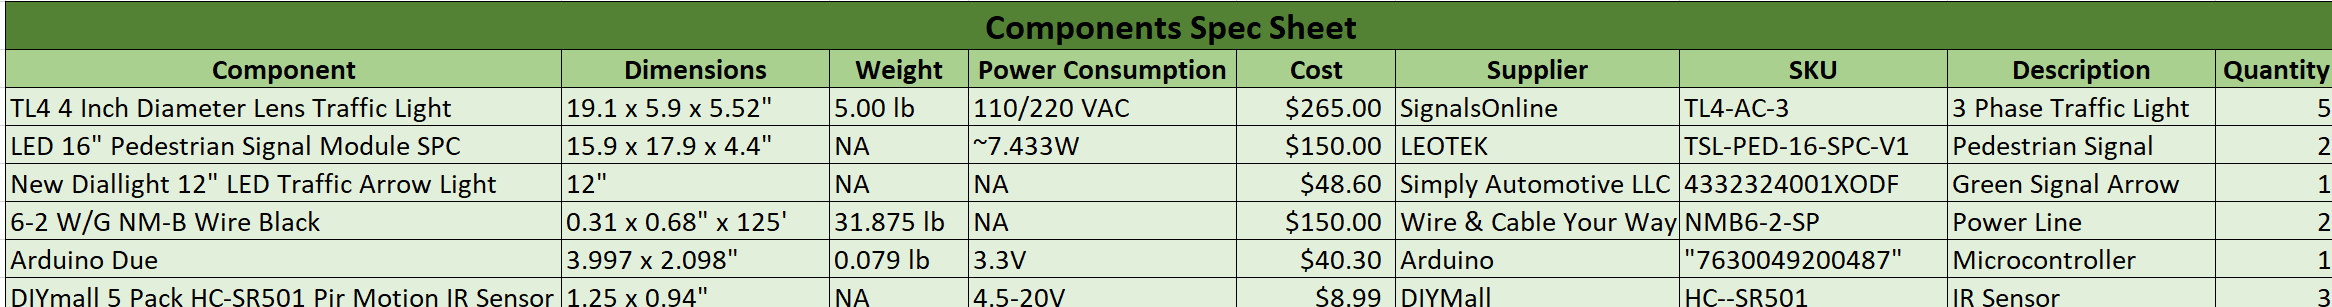
\includegraphics[width=\textwidth, center]{SpecChart.png}
\scriptsize{
Figure 9: Specifications Chart.
}
\end{center}

The total cost of all of the components is $ \$2,040.87$. All components may be purchased and shipped online. 

\section{Summary}
Using the ideas of States, Conditions, Transitions, and Sequences, a traffic control system can be developed for the crosswalk on Eighth Street, between Sundquist and Maynard. This system takes into account the idea that the pedestrian should not wait longer than 60 seconds, and their should not be any traffic jam at the College Street or Joseph Street intersections. It also takes into account the Trahern lot influx.

To implement this system, Traffic Lights, Pedestrian Lights, an Arduino, and Inferred Sensors are used to intake the situation, and output a proper traffic control response. AutoCAD and Google Maps were used to produce a site map of the surrounding area, which is helpful with understanding the flow of traffic as well as helping with the installation process.



\end{document}